\subsubsection*{Esercizio 11.2 pag. 246 Hoff}

Randomized block design: researchers interested in identifying the optimal planting density for
a type of perennial grass performed the following randomized experiment: ten different plots of
land were each divided into eight subplots, and planting densities of 2, 4, 6 and 8 plants per
square meter were randomly assigned to the subplots, so that there are two subplots at each
density in each plot. At the end of the growing season the amount of plant matter yield was
recorded in metric tons per hectare. These data appear in the file pdensity.dat. The researchers
want to fit a model like $y = \beta_1 + \beta_2 x + \beta_3 x^2 + \epsilon$, where $y$ is yield and $x$ is planting density,
but worry that since soil conditions vary across plots they should allow for some across-plot
heterogeneity in this relationship. To accommodate this possibility we will analyze these data
using the hierarchical linear model described in Section 11.1.

\begin{enumerate}
    \item Before we do a Bayesian analysis we will get some ad hoc estimates of these parameters via
    least squares regression. Fit the model $y = \beta_1 +\beta_2 x+\beta_3 x^2 + \epsilon$ using OLS for each group,
    and make a plot showing the heterogeneity of the least squares regression lines. 
    From the least squares coefficients find ad hoc estimates of $\theta$  and $\Sigma$. 
    Also obtain an estimate of $\sigma$ 2 by combining the information from the residuals across the groups.
    \item Now we will perform an analysis of the data using the following distributions as prior distributions:
    $$ \Sigma^{-1} \sim \text{Wishart}(4, \hat\Sigma^{-1})$$
    $$ \theta \sim \text{multivariate normal} (\hat\theta, \hat\Sigma)$$
    $$ \sigma^2 \sim \text{inverse-gamma}(1, \hat\sigma^2)$$

    where $\hat\theta,|\hat\Sigma, \sigma^2 $ are the estimates you obtained in a). 
    Note that this analysis is not combining prior information with information from the data, as the “prior” distribution is based on
    the observed data. 
    However, such an analysis can be roughly interpreted as the Bayesian
    analysis of an individual who has weak but unbiased prior information.
    
    \item Use a Gibbs sampler to approximate posterior expectations of $\beta$ for each group $j$, and plot
    the resulting regression lines. Compare to the regression lines in a) above and describe why
    you see any differences between the two sets of regression lines.

    \item From your posterior samples, plot marginal posterior and prior densities of $\theta$ and the
    elements of $\Sigma$. 
    Discuss the evidence that the slopes or intercepts vary across groups.
    \item Suppose we want to identify the planting density that maximizes average yield over a
    random sample of plots. 
    Find the value $x_max$ of x that maximizes expected yield, and
    provide a 95\% posterior predictive interval for the yield of a randomly sampled plot having
    planting density $x_max$.
\end{enumerate}

\subsubsection*{Premessa e indicazioni generali}
L'esercizio ha in generale l'obiettivo di valutare la relazione tra raccolto e densità di piante
relativamente a 10 lotti di terra su cui sono stati osservati i dati secondo il seguente disegno a
blocchi randomizzato:

\begin{itemize}
    \item 10 lotti di terra.
    \item Ogni lotto è diviso a sua volta in 8 sottolotti.
    \item Densità di piantagione pari a 2, 4, 6 e 8 sono assegnate in maniera casuale tra
    gli 8 sottolotti di ogni lotto: in questo modo ogni lotto ha due sottolotti di ognuna delle quattro densità.
\end{itemize}

È richiesta 'analisi della relazione tra raccolto e densità mediante un modello di regressione
lineare quadratica e tenendo conto della variabilità tra gruppi in termini di condizioni di suolo.
Per come è costruito il disegno e per come è formulato il modello procediamo nel'analisi attraverso
un modello di regressione lineare gerarchico. Il setting del modello è:\\
$ Y_{ij} = \underset{1*p p * 1}{\beta^T_jx_{ij}} + \epsilon_{ij} \qquad \qquad \epsilon_{ij}|\sigma^2 \sim i.i.d. N(0,\sigma^2)$
\\
o equivalentemente 
\begin{description}[leftmargin=6.8cm]
    \item [$ \underset{n_j *1}{Y_j} | \underset{p * 1}{\beta_j}, \underset{n_j * p}X_j, \sigma^2 \sim N_{n_j} (\underset{n_j*p p*1}{X_j \beta_j}, \sigma^2 \underset{n_j nj}{I})$]
    $i = 1, \dots, n; j = 1, \dots, m.$ 

    Modello che descrive la variabilità all'interno di ogni gruppo.
\end{description}
$ Y_i \perp Y_j | \beta_1, \dots, \beta_m, \sigma^2 i \neq j$ \\
\begin{description}[leftmargin=5cm]
    \item [$ \underset{p *1}{\beta_j} | \underset{p * 1}{\theta}, \underset{p * p}\Sigma \sim i.i.d. N_{p} (\underset{p*1}{\theta}, \underset{p *p }{\Sigma})$]
    Modello che descrive la variabilità tra gruppi.
\end{description}
$ \underset{p *1}{\theta} | \underset{p * p}{\mu_0}, \underset{p * p}{\Lambda_0} \sim N_p(\underset{p*1}{\mu_0}, \underset{p * p}{\Lambda_0}) $
\begin{description}[leftmargin=6.2cm]
    \item [$ \underset{p * p}{\Sigma} \sim \text{\normalfont{Inverse - Wishart}}(\eta_0, \underset{p*1}{S_0{-1}})$]
    Prior semiconiugate: è possibile fare inferenza approssimando la distribuzione congiunta a posteriori \\
    $p(\sigma^2, \theta,\beta_1, \dots, \beta_m, \Sigma|X_1, \dots, X_m, y_1,\dots, y_m)$
    mediante Gibbs sampler.
\end{description}
$ \sigma^2 | v_0, \sigma^2_0\sim \text{\normalfont{Inverse - Gamma}}(\frac{v_0}{2}, \frac{v_0\sigma^2_0}{2})$
\\
Per il DAG si faccia riferimento al grafo dell'esercizio precedente.
Riportiamo adesso il codice R con output e commenti necessari per rispondere ai quesiti dell'esercizio.

\begin{lstlisting}[style=R]
#Funzione per campionare da una normale multivariata:
rmvnorm<-
function(n,mu, Sigma ) {
    p<-length(mu)
    res<-matrix ( 0, nrow=n, nco l=p)
    if ( n>0 & p>0 ) {
        E<-matrix( rnorm(n*p),n, p)
        res<-t ( t (E%*%chol ( Sigma ) ) +c (mu) )
        #R <- chol(A)
}
res
}

#Funzione per campionare da una Wishart:
rwish<-function (n, nu0, S0 )
{
    sS0 <- cho l ( S0 )
    S<-array ( dim=c ( dim( S0 ),n ) )
    for ( i in 1: n)
    {
        Z <-matrix ( rnorm( nu0 * dim( S0 ) [ 1 ] ), nu0, dim( S0 ) [ 1 ] ) %*% sS0
        + S [,, i ]<-t (Z)%*%Z
    }
    S [,, 1: n ]
}

#Funzione per campionare da una Inverse-Wishart:

rinvwish<-function(n, nu0, iS0 )
{
    sL0 <- cho l ( iS0 )
    S<-array ( dim=c ( dim( iS0 ),n ) )
    for ( i in 1: n)
{
    Z <- matrix ( rnorm( nu0 * dim( iS0 ) [ 1 ] ), nu0, dim( iS0 ) [ 1 ] ) %*% sL0
    S [,, i ]<- solve ( t (Z)%*%Z)
}
    S [,, 1: n ]
}

#Lettura dei dati:

dati<-read.table("C:\\Desktop\\pdensity.dat", header=TRUE)
> head (dati)


\end{lstlisting}
{
\color{red}
\begin{Verbatim}
plot density yield
1       2     8.25
1       2     5.81
1       4     8.69
1       4     8.03
1       6     7.96
1       6     8.89
\end{Verbatim}
}

\begin{lstlisting}[style=R]
#Calcolo di quantita' utili per ogni gruppo ( numerosita', vettore delle osservazioni, matrice del modello e numero di parametri ):
ids<-unique (datis$plot )
m<-length ( ids )
Y<-list() ; X<-list() ; N<-NULL
for ( j in 1:m)
{
    Y[ [ j ]]<-dati [ dati [,1]== ids [ j ], 3]
    N[ j]<- sum( dati$plot==ids [ j ])
    xj<-dati [ dati [,1]== ids [ j ], 2]
    X[ [ j ]]<-cbind ( rep (1,N[ j ]), xj, xj^2 )
}
p<-dim(X[ [ 1 ] ] ) [2]
N
\end{lstlisting}

{
\color{red}
\begin{verbatim}
[1] 8 8 8 8 8 8 8 8 8 8
\end{verbatim}
}

\begin{lstlisting}[style=R]
Y[ [ 1 ] ]
\end{lstlisting}

{
\color{red}
\begin{verbatim}
[1] 8.25 5.81 8.69 8.03 7.96 8.89 6.13 9.40    
\end{verbatim}
}

\begin{lstlisting}[style=R]
X[ [ 1 ] ]
\end{lstlisting}

{
\color{red}
\begin{verbatim}
     xj
[1,] 1 2 4
[2,] 1 2 4
[3,] 1 4 16
[4,] 1 4 16
[5,] 1 6 36
[6,] 1 6 36
[7,] 1 8 64
[8,] 1 8 64
\end{verbatim}
}

\begin{lstlisting}[style=R]
#a )
#Stimiamo i coefficienti di regressione secondo il metodo OLS
#indipendentemente in ciascuno de i 10 lotti:
S2.OLS<-BETA.OLS<-NULL
for( j in 1:m) {
    fit<-lm(Y[ [ j ]]~-1+X[ [ j ] ] )
    BETA.OLS<-rbind (BETA.OLS, c ( fit$coef ) )
    S2.OLS<-c ( S2.OLS, summary( fit )$sigma ^2)
}

colnames (BETA.OLS)<-c ("1"," x "," x^2")
> BETA.OLS
\end{lstlisting}

{
\color{red}
\begin{Verbatim}
            1       x         x^2
[1,]    4.84000 1.357250 -0.1243750
[2,]    4.53375 1.193375 -0.1290625
[3,]    2.07750 2.128250 -0.1643750
[4,]    2.60375 2.114875 -0.1928125
[5,]    3.57000 1.540500 -0.1500000
[6,]    1.47375 1.930875 -0.1215625
[7,]    3.96375 1.424875 -0.1278125
[8,]    0.52375 2.941875 -0.2653125
[9,]    3.36250 1.675500 -0.1400000
[10,]   1.73875 2.241125 -0.1771875
\end{Verbatim}
}

\begin{lstlisting}[style=R]
S2.OLS
\end{lstlisting}

{
\color{red}
\begin{Verbatim}
[1] 1.8005320 1.0760545 0.8134580 0.5019505 0.5886680 0.8074545 0.9575905
[8] 0.3965025 0.1328380 0.8030505
\end{Verbatim}
}



\begin{lstlisting}[style=R]
#Rappresentiamo graficamente le 10 linee di regressione per valutare la variabilita' tra gruppi. Riportiamo sul grafico anche la loro media.

par (mfrow=c (1,2) )
plot ( range ( dati [,2]), range ( dati [,3]), type="n", xlab="planting density ", +ylab="Expected yield ",main="Regression lines OLS")
for ( j in 1:m) {curve (BETA.OLS[ j,1]+BETA.OLS[ j,2]* x+BETA.OLS[ j,3]* x^2,
col="gray ",add=T)}
BETA.OLS.MEAN<-apply (BETA.OLS,2,mean)
curve (BETA.OLS.MEAN[1]+BETA.OLS.MEAN[2]* x+BETA.OLS.MEAN[3]* x^2,lwd=2,add=T)

BETA.OLS.MEAN
\end{lstlisting}

\begin{figure}
    \centering
    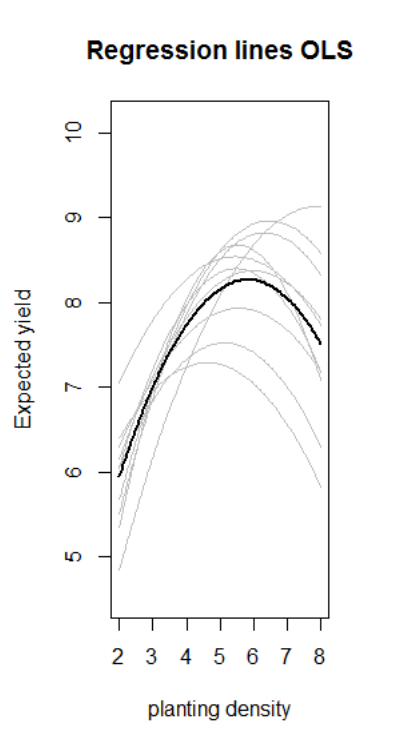
\includegraphics[totalheight=8cm]{img/esercizio11-2-1.png}
    \caption{ Curve di regressione con stime OLS.}
\end{figure}

{
\color{red}
\begin{Verbatim}
    1       x       x^2
2.86875 1.85485 -0.15925
\end{Verbatim}
}

\begin{lstlisting}[style=R]
cov(BETA.OLS)
\end{lstlisting}

{
\color{red}
\begin{Verbatim}
        1           x           x^2
1 2.00120764    -0.69321313  0.044309549
x -0.69321313    0.27555421 -0.020742679
x 2 0.04430955  -0.02074268  0.001968451
\end{Verbatim}
}

\begin{lstlisting}[style=R]
mean(S2.OLS)
\end{lstlisting}

{
\color{red}
\begin{Verbatim}
[1] 0.7878099
\end{Verbatim}
}

\begin{lstlisting}[style=R]
#Si osserva che:
#-)Tutte le curve hanno lo stesso andamento quadratico: crescente fino ad una densita' di piante pari circa a 6 e poi decrescente.
#-)Alcuni gruppi si discostano particolarmente dalla media generale: il raccolto medio risulta o molto inferiore o molto superiore, soprattutto per i valori piu' grandi del range della covariata. Nel caso in cui i lotti avessero diverse numerosita' al loro interno potremmo immaginare che questo si verifica per i lotti meno numerosi ; in realta' per come e' disegnato l' esperimento questa variabilita' osservata e' dovuta ad altro, forse alle diverse condizioni del terreno dei 10 appezzamenti.

#b)

#Setting delle prior: impostiamo le prior semiconiugate per theta, Sigma e sigma2 come richiesto. Ricordiamo che le prior sono specificate in ottica empirico-bayesiana e che quindi l' analisi non combina le informazioni a priori con quelle a posteriori ma puo' essere all' incirca interpretata come quella di un individuo con informazione debole ma non distorta.
theta<-BETA.OLS.MEAN; Sigma<-cov(BETA.OLS) ; sigma2<-mean(S2.OLS)
eta0 <-4; S0<-Sigma
mu0<-theta ; L0<-Sigma
v0<-2; sigma20<-sigma2

#c)

#Impostiamo come richiesto un Gibbs sampler: infatti e' possibile approssimare in questo modo la distribuzione a posteriori dal momento che usiamo prior semiconiugate. Per le distribuzioni full conditional si veda il quaderno.
#Numero di simulazioni:

nsimul=10000

#Valori iniziali dei parametri:

beta<-BETA.OLS
Sigma<-cov(BETA.OLS)
sigma2<-mean(S2.OLS)

#Oggetti in cui inseriamo durante l' algoritmo i valori campionati dalle full conditional:

Sigma.post<-matrix (0,p,p)
BETA.pp<-THETA.POST<-S2.POST<-NULL
BETA.POST<-BETA.OLS*0
SIGMA.POST<-array (0, c(p,p, nsimul ) )
set.seed (1)

#Algoritmo Gibbs per nsimul iterazioni
for ( s in 1: nsimul ) {
    for ( j in 1:m)
    {
        #Per ogni gruppo campioniamo i coefficienti di regressione:

        Vj<-solve ( solve (Sigma) + t (X[ [ j ] ] )%*%X[ [ j ]]/ sigma2 )
        Ej<-Vj%*%( solve (Sigma)%*%theta + t (X[ [ j ] ] )%*%Y[ [ j ]]/ sigma2 )
        beta [ j,]<-rmvnorm(1,Ej, Vj)
    }

    #Campioniamo la supermedia theta dei coefficienti di regressione:
    Lm<- solve ( solve (L0) + m* solve (Sigma) )
    mum<- Lm%*%( solve (L0)%*%mu0 + solve (Sigma)%*%apply ( beta,2,sum) )
    theta<-t (rmvnorm(1,mum,Lm) )

    #Campioniamo la matrice di varianza e covarianza Sigma dei coefficienti di regressione:
    mtheta<-matrix ( theta,m,p, byrow=TRUE)
    Sigma<-solve ( rwish (1, eta0+m, solve ( S0+t ( beta-mtheta)%*%(beta-mtheta) ) ) )
    #Campioniamo la varianza residua:

    RSS<-0
    for ( j in 1:m) { RSS<-RSS+sum( (Y[ [ j ]]-X[ [ j ]]%*%beta [ j, ] )^2 ) }
    sigma2<-1/rgamma(1,( v0+sum(N) ) /2, (v0*sigma20+RSS)/2 )
    #Immagazziziniamo i valori appena campionati:
    S2.POST<-c(S2.POST, sigma2 ) ;THETA.POST<-rbind (THETA.POST, t ( theta ) )
    Sigma.post<-Sigma.post+Sigma ; BETA.POST<-BETA.POST+beta
    SIGMA.POST[,, s]<-Sigma
    #Campioniamo dalla posterior predictive dei coefficienti di regressione che ci servira' per il punto e).
    BETA.pp<-rbind (BETA.pp,rmvnorm(1, theta, Sigma) )
}
colnames (THETA.POST)<-c(" theta1 "," theta2 "," theta3 ")
colnames (BETA.POST)<-colnames (BETA. pp)<-c(" beta1 "," beta2 "," beta3 ")

#Plottiamo adesso le curve di regressione con le stime dei coefficienti derivanti dal Gibbs sampler per poi confrontarle con quelle precedenti in caso di stima OLS. Anche in questo caso la media delle curve e' di colore nero.

BETA.PM<-BETA.POST/nsimul
plot ( range (c (0,10) ), range (c (0,10) ), type="n",
xlab="planting density ", ylab="Yield ",main="Bayesian regression lines ")
for ( j in 1:m) { curve (BETA.PM[ j,1]+BETA.PM[ j,2]* x+BETA.PM[ j,3]* x^2,
col="gray ",add=T)}
curve ( mean(THETA.POST[,1])+mean(THETA.POST[,2]) *x+
mean(THETA.POST[,3]) *x^2,lwd=2,add=T )
#dev.off ()

#Osservando i due grafici a confronto si nota che il modello gerarchico permette di trarre informazioni dai gruppi, riportando le curve di regressione lungo la media. In particolare vediamo adesso che l' andamento delle curve e' ancora piu' simile rispetto al caso OLS e che per valori piu' grandi del range di x il valore atteso del raccolto e' si' sempre piu' basso in alcuni casi e sempre piu' alto in a l t r i rispetto alla media, ma con un' intensita' minore. Dal momento che lavoriamo con gruppi tutti di piccola numerosita' c' e' una grande variabilita' nelle stime OLS mentre nel caso del modello gerarchico i gruppi si influenzano in termini di informazioni e per l' effetto di shrinkage la stima OLS viene portata verso la stima media in modo uguale per mtutti i gruppi perche' hanno la stessa numerosita' campionaria.

#Controlliamo la convergenza dell' algoritmo:

library (coda)
effectiveSize (THETA.POST)
\end{lstlisting}

\begin{figure}
    \centering
    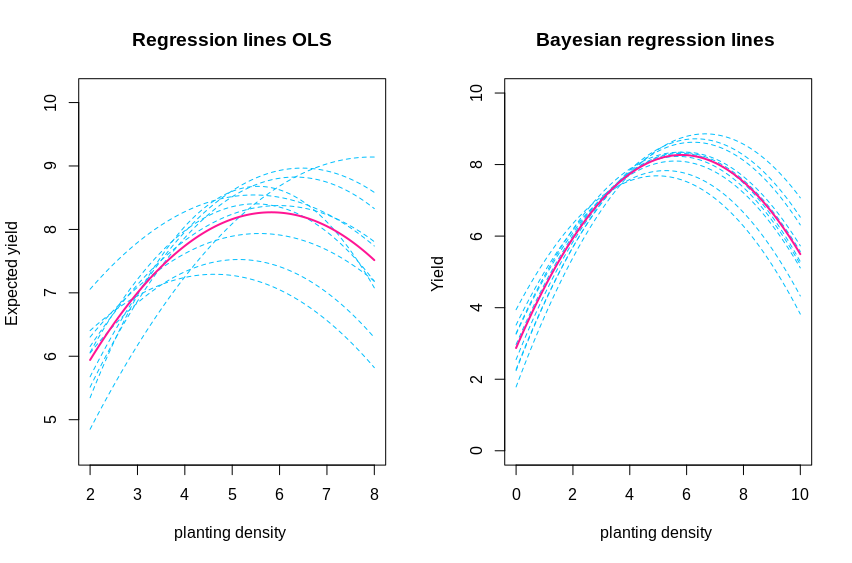
\includegraphics[totalheight=8cm]{img/esercizio11-2-2.png}
    \caption{ GLMM: stime dei minimi quadrati e stime bayesiane a confronto.}
\end{figure}
\newpage
{
\color{red}
\begin{Verbatim}
theta1      theta2   theta3
1009.3091 742.6614 656.8365
\end{Verbatim}
}

\begin{lstlisting}[style=R]
#d)

#Approssimazione delle distribuzioni a priori tramite simulazione Monte Carlo ( facciamo notare che potremmo derivarle anche analiticamente ):

n<-10000

THETA.PRIOR<-rmvnorm(n,mu0,L0) ; colnames (THETA.PRIOR)<-colnames (THETA.POST)
SIGMA.PRIOR<-rinv
head(THETA.PRIOR)
\end{lstlisting}

\newpage
{
\color{red}
\begin{Verbatim}
           theta1      theta2     theta3
[1,]  -1.77780314    3.529232 -0.2613000
[2,]   3.47065885    1.752018 -0.1395134
[3,]   3.60717709    1.583506 -0.1350985
[4,]   0.07323521    2.928965 -0.2604753
[5,]   3.05388848    1.832459 -0.1571405
[6,]   2.27382048    1.786574 -0.1183835
\end{Verbatim}
}

\begin{lstlisting}[style=R]
head(SIGMA.PRIOR)
\end{lstlisting}

{
\color{red}
\begin{Verbatim}
[1] 3.63026418 -0.93710237 0.04650011 -0.93710237 0.28263581 -0.01833983
\end{Verbatim}
}

\begin{lstlisting}[style=R]
#A priori e a posteriori di theta a confronto ( plot ):

par (mfrow=c (2,2) )
for ( i in 1:3) {
    plot ( density (THETA.POST[, i ]), xlab=paste (" theta ", i ),main="")
    lines ( density (THETA.PRIOR[, i ]), col="grey ")
    legend (" topright ", legend=c(" Prior "," Posterior "), col=c(" grey "," black "),
    lty =1,bty="n", cex =0.7)
}
\end{lstlisting}

\begin{figure}
    \centering
    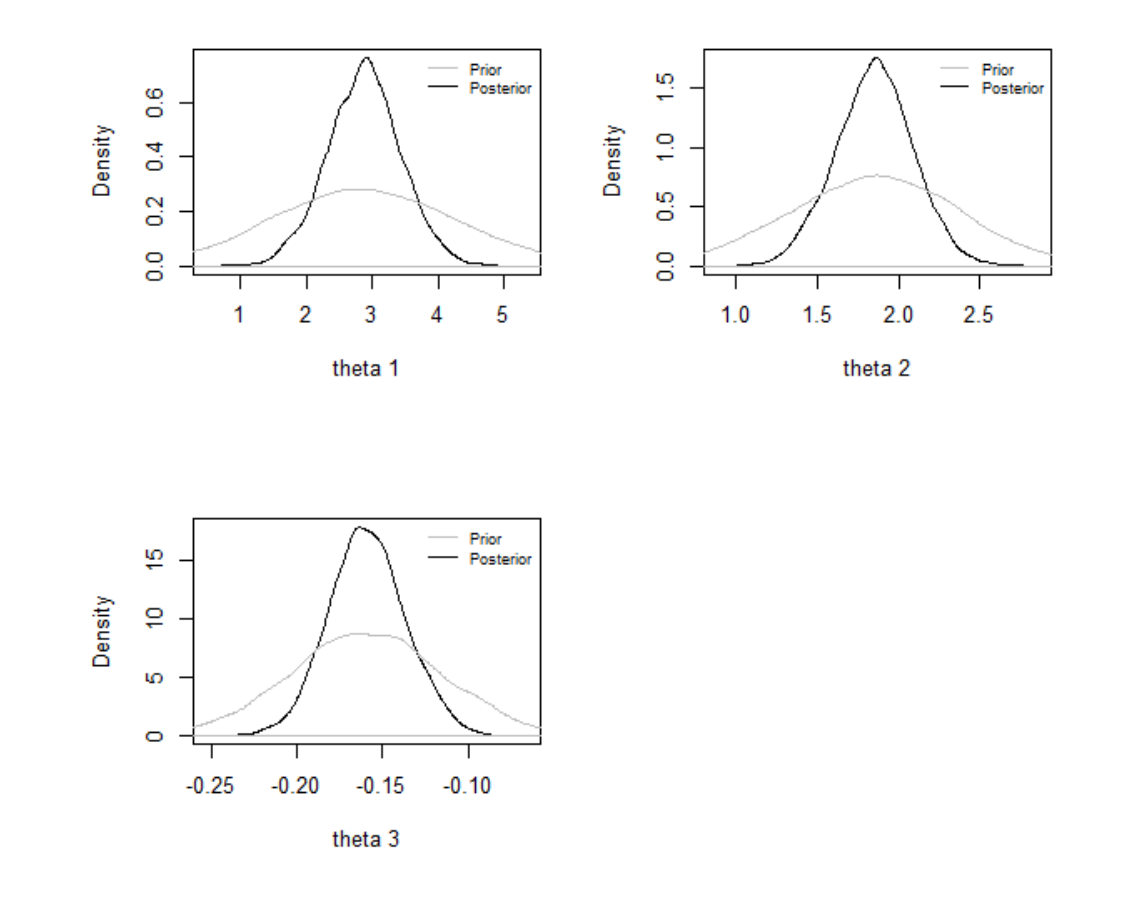
\includegraphics[totalheight=8.5cm]{img/esercizio11-2-3.png}
    \caption{  Densità a priori e a posteriori a confronto (media).}
\end{figure}

\begin{lstlisting}[style=R]
#Si osserva che le distribuzioni a posteriori, pur essendo centrate sulla stessa media delle a priori (come ci aspettavamo dal momento che abbiamo centrato le prior nelle stime di massima verosimiglianza ), sono meno diffuse: in questo modo l' informazione a posteriori cambia nel senso che si da' maggiore probabilita' ai valori che cadono attorno ad essi.

#Prior e posterior di Sigma a confronto ( plot ):

par (mfrow=c (2,2) )
for ( i in 1:3) {
plot ( density ( log (SIGMA.POST[ i, i, ] ) ), type="l ", xlab=paste ("Sigma", i ),
ylab="density ",main="")
lines ( density ( log (SIGMA.PRIOR[ i, i, ] ) ), col="gray ",lwd=2)
legend (" topright ", legend=c(" Prior "," Posterior "), col=c(" gray "," black "),
bty="n", lty=1)
}

#NB Abbiamo preso il logaritmo degli elementi di Sigma dal momento che sono valori molto bassi. NB Dal momento che e' richiesto di commentare la variabilita' relativa all' intercetta e alle pendenze nei gruppi, riportiamo i plot delle distribuzioni dei soli elementi della diagonale principale di Sigma.Commento al plot: ' e' evidenza che la variabilita' tra i gruppi delle intercette non e' molto elevata, ma diminuisce ancora per il primo e per il secondo coefficiente ( ricordiamo che dal momento che consideriamo il logaritmo delle varianze la variabilita' e' minore e' indicata da una densita' concentrata su valori sempre piu' negativi.

#e)

#Si vuole trovare la densita' di piante che massimizza il raccolto atteso per un campione di lotti. Ricordiamo che stiamo lavorando con un modello gerarchico e quindi vogliamo tenere in considerazione anche la variabilita' tra gruppi: ci serviamo a questo scopo della distribuzione predittiva a posteriori dei coefficienti di regressione (una normale multivariata con vettore delle medie e matrice di varianza e covarianza pari quelli estratti ad ogni passo dell' algoritmo ) per cui ogni vettore di coefficienti estratto rappresenta il vettore dei coefficienti di regressione per un gruppo futuro. Disponiamo gia' di tale distribuzione dal momento che e' stata calcolata durante l' algoritmo. ' necessario adesso confrontare 4 distribuzioni: quelle dei valori attesi del raccolto di un generico lotto, una per ogni valore osservato della covariata x. Anche in questo caso vogliamo tenere in considerazione la variabilita' tra lotti e per questo approssimiamo le distribuzioni usando la predittiva a posteriori dei coefficienti di regressione appena discussa. Cerchiamo il valore atteso di y date le y passate e le x. Un modo per farlo e' campionare i beta dalla loro posterior predictive e capionare le y dati i valori della x e quindi per ogni valore della x potevamo avere un valore atteso. Facciamo la media delle distribuzioni dei valori attesi. Campioniamo i beta tilde: i beta per un gruppo futuro. Per ogni valore di questo beta campinato abbiamo un valore del valore atteso per un y futuro. Alla fine per ogni x si genera una distribuzione del valore atteos della y futuro (4 vettori ). Confrontiamo le 4 distribuzioni ( per es con la media o vedendo la prob. che una sia maggiore dell' altra ). Prendendo il valore medio per ogni valore di beta tilde e per l' ixmax e la varianza a posteriori campiono un valore y. Cosi' si incorpora anche l' incertezza derivante dai gruppi.

x0<-c (2,4,6,8)
raccolto<-NULL
for ( i in x0){
x<-c (1, i, i ^2)
raccolto<-cbind ( raccolto,BETA. pp%*%x)
}
colnames ( raccolto )<-x0
head( raccolto )
\end{lstlisting}


\begin{figure}
    \centering
    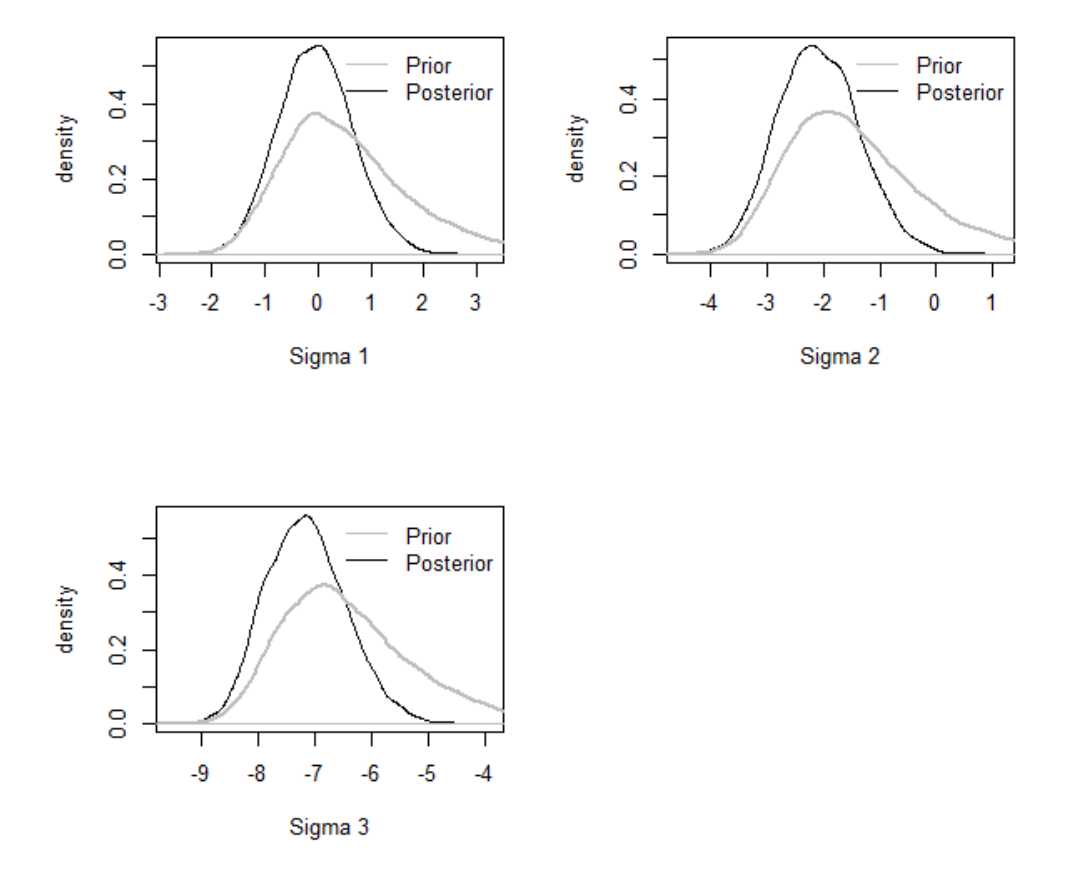
\includegraphics[totalheight=10cm]{img/esercizio11-2-4.png}
    \caption{  Densità a priori e a posteriori a confronto (variabilità e covariabilità).}
\end{figure}

{
\color{red}
\begin{Verbatim}
            2        4        6        8
[1,] 5.989406 7.758386 8.317531 7.666840
[2,] 6.033526 7.921516 8.605911 8.086712
[3,] 6.350655 7.597301 7.712147 6.695192
[4,] 6.888414 7.776763 7.907158 7.279599
[5,] 5.973396 7.669427 8.482208 8.411740
[6,] 6.247427 7.685203 7.955526 7.058398
\end{Verbatim}
}

\begin{lstlisting}[style=R]
#Confrontiamo adesso le quattro distribuzioni dei valori attesi,
#graficamente e con un indice sintetico, la media:

par (mfrow=c (1,1) )
hist ( raccolto [,1], prob=T, main="Raccolto atteso a posteriori ", xlab="Raccolto ",
xlim=c (2,13), ylim=c (0,1.5) )
lines ( density ( raccolto [,1]) )
hist ( raccolto [,2], prob=T, col="red ",add=T)
lines ( density ( raccolto [,2]), col="red ")
hist ( raccolto [,3], prob=T, col="green ",add=T)
lines ( density ( raccolto [,3]), col="green ")
hist ( raccolto [,4], prob=T, col="blue ",add=T)
lines ( density ( raccolto [,4]), col="blue ")
legend (" topright ", legend=c("x=2","x=4","x=6","x=8"), col=c(" black "," red ",
"green "," blue "), lty=1)
apply ( raccolto,2,mean)
\end{lstlisting}

{
\color{red}
\begin{Verbatim}
       2        4        6        8
5.942984 7.739188 8.264142 7.517844
\end{Verbatim}
}

\begin{figure}
    \centering
    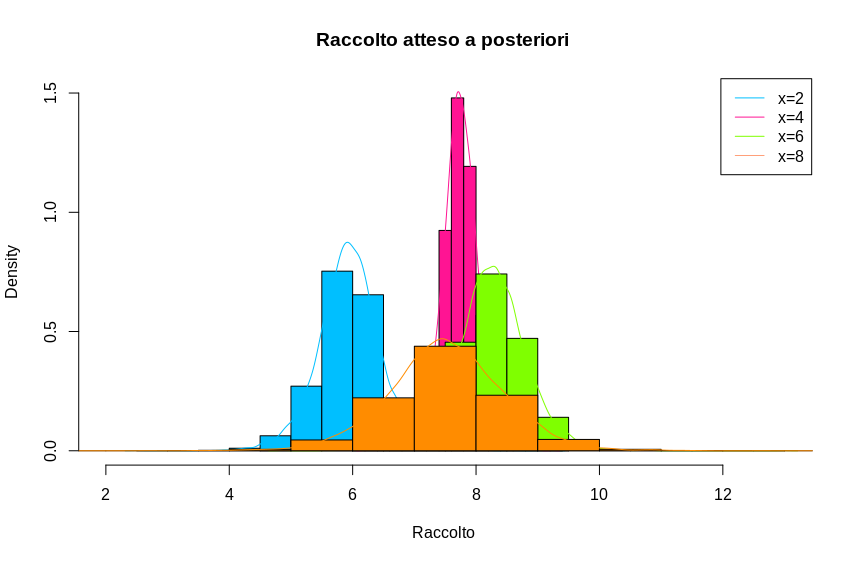
\includegraphics[totalheight=8cm]{img/esercizio11-2-5.png}
    \caption{  Valori attesi a posteriori per più valori di x a confronto.}
\end{figure}

\begin{lstlisting}[style=R]
#Si osserva che il valore della covariata che masimizza il raccolto atteso per un generico lotto e' x=6. Procediamo quindi considerando tale valore per il predittore lineare. Si vuole infine approssimare la distribuzione predittiva a posteriori per un generico lotto avendo una densita' di piantagioni pari a 6. La logica e' la stessa di quella usata per la predittiva a posteriori dei coefficienti di regressione, con la differenza che adesso siamo al livello piu' basso della gerarchia e quindi si aggiunge un parte di variabilita' dovuta alle osservazioni campionarie. Per ogni vettore dei coefficienti estratto dalla predittiva a posteriori e per ogni elemento estratto dalla a posteriori della varianza residua ( anche questo fatto gia' fatto nell' algoritmo ) campioniamo un valore del raccolto da una normale con media pari al predittore lineare e varianza pari alla varianza residua. Riportiamo infine un plot della densita' e l' intervallo di confidenza richiesto per tale distribuzione:

y. pred<-rnorm( nsimul,BETA. pp%*%x, S2.POST)
quantile (y. pred, c (0.025,0.975) 
\end{lstlisting}


{
\color{red}
\begin{Verbatim}
    2.5%    97.5%
5.213170 9.855576
\end{Verbatim}
}

\begin{lstlisting}[style=R]
hist (y. pred, prob=T, main="Predittiva a posteriori ", xlab="raccolto ")
lines (y. pred )
\end{lstlisting}

\begin{figure}
    \centering
    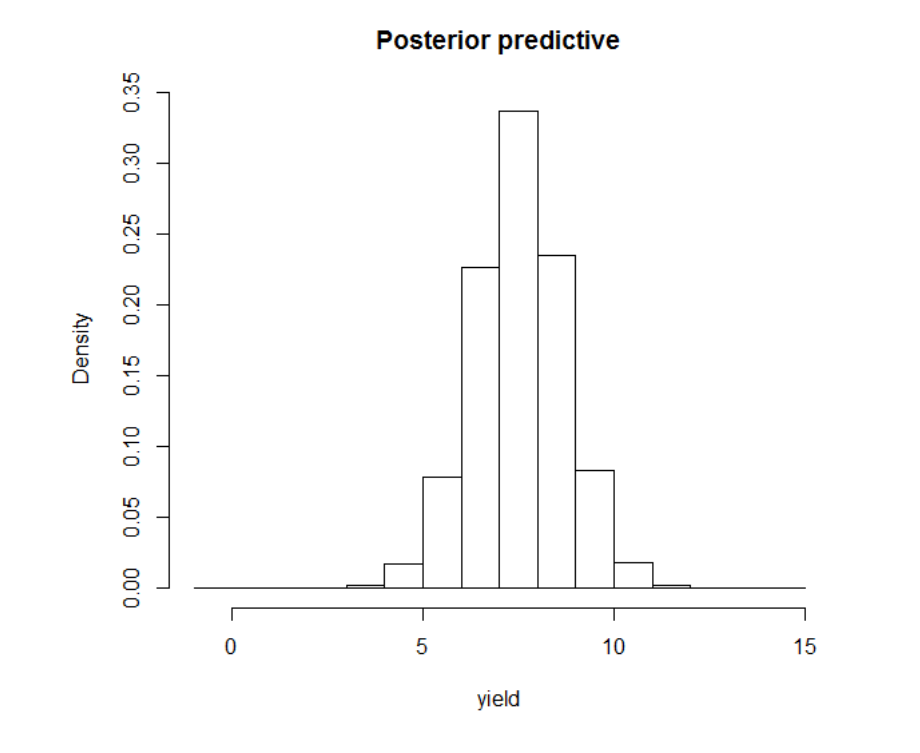
\includegraphics[totalheight=10cm]{img/esercizio11-2-6.png}
    \caption{   Predittiva a posteriori.}
\end{figure}